
\documentclass{beamer}

\mode<presentation>{\usetheme{Madrid}}

\usepackage[utf8]{inputenc}
\usepackage[ngerman]{babel}
\usepackage{amsmath, amssymb, amsthm}
\usepackage{graphicx}
\usepackage{booktabs}
\usepackage{tikz}
\usetikzlibrary {automata}
\usepackage{stmaryrd}

\usepackage{subcaption}


\author[Philipp Geier]{}
\title[Sorting Colored Balls in Colored Tubes]{Sorting Colored Balls in Colored Tubes \\ von Ernst Althaus et. al}
\institute[Universität Trier]{}
\date{}
\beamertemplatenavigationsymbolsempty

\usepackage{enumitem}
\newlist{arrowlist}{itemize}{1}
\setlist[arrowlist]{label=$\Rightarrow$}
\newlist{pointlist}{itemize}{1}
\setlist[pointlist]{label=$\circ$}
\newlist{enumlist}{enumerate}{1}
\setlist[enumlist]{label=\arabic*.}

%—-------------------------------------------------------------

\begin{document}
{
  \usebackgroundtemplate{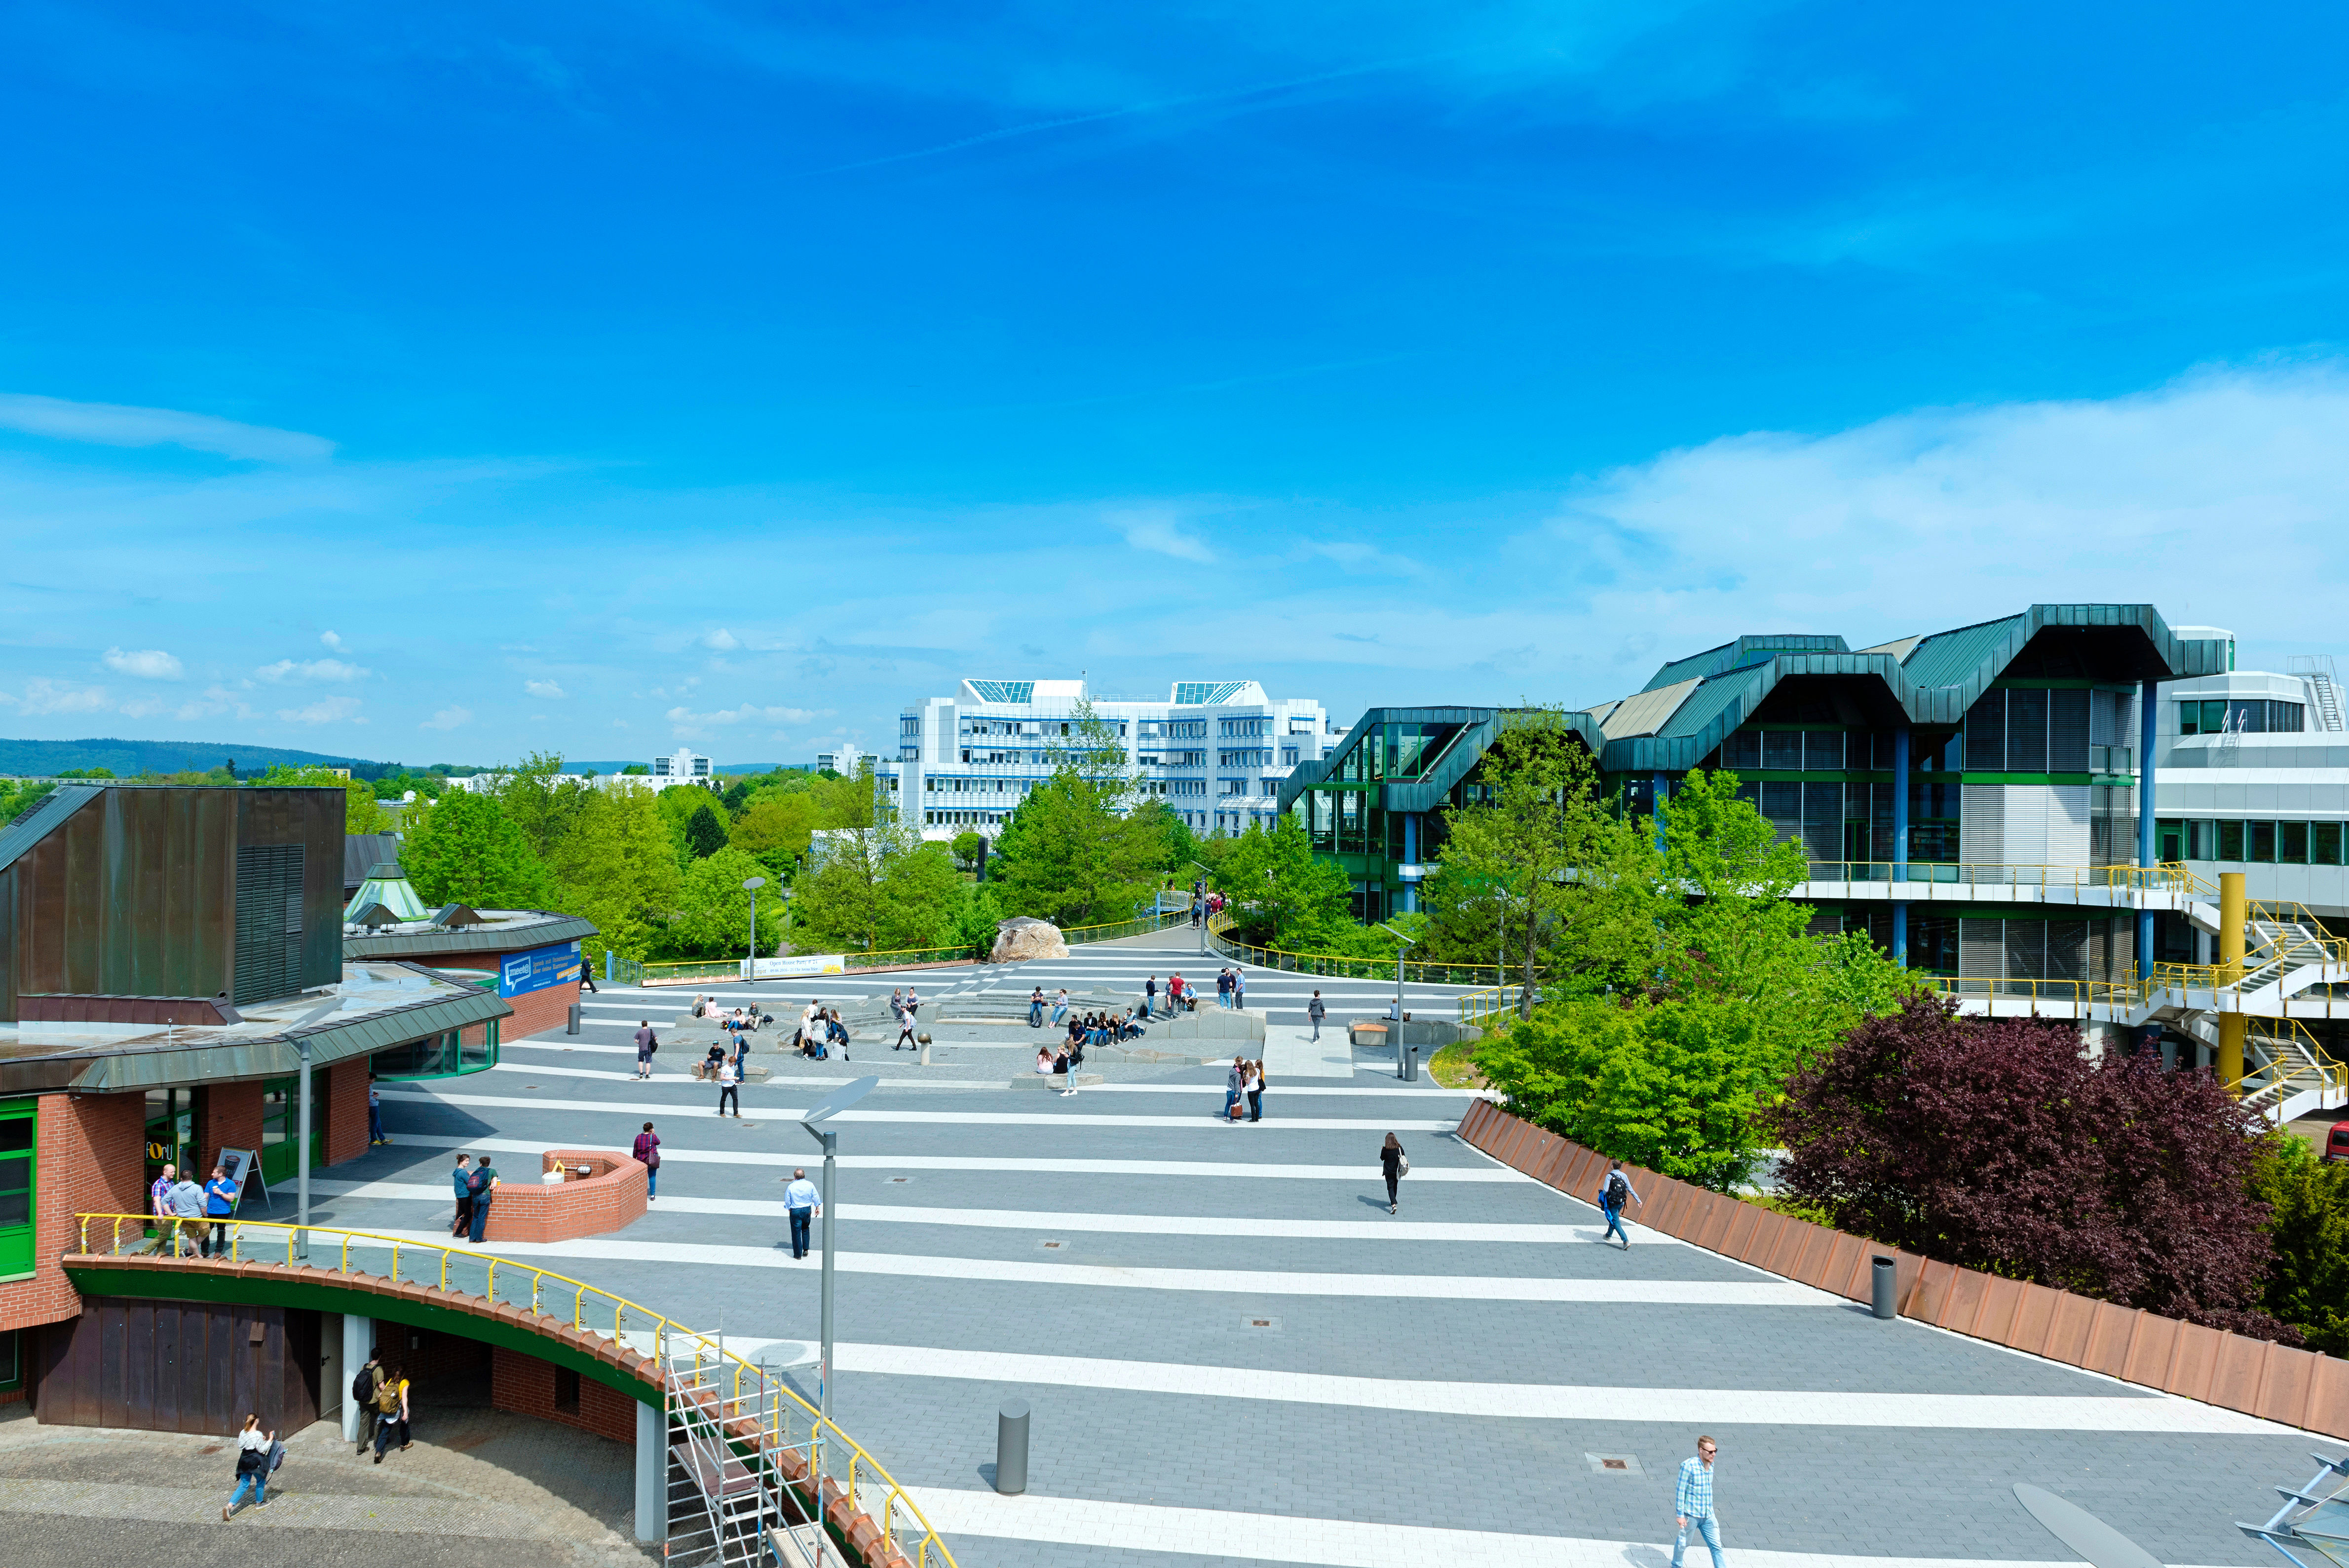
\includegraphics[width=1.2\paperwidth]{unitrier}}
  \begin{frame}
    \maketitle
  \end{frame}
}
    
    %\begin{frame}
       % \frametitle{Inhalt}
		%\tableofcontents
	%\end{frame}
	
%—------------------------------------------------------


\begin{frame}{Ziel: Kleinste Anzahl an Zügen}
	\begin{figure}[ht]
		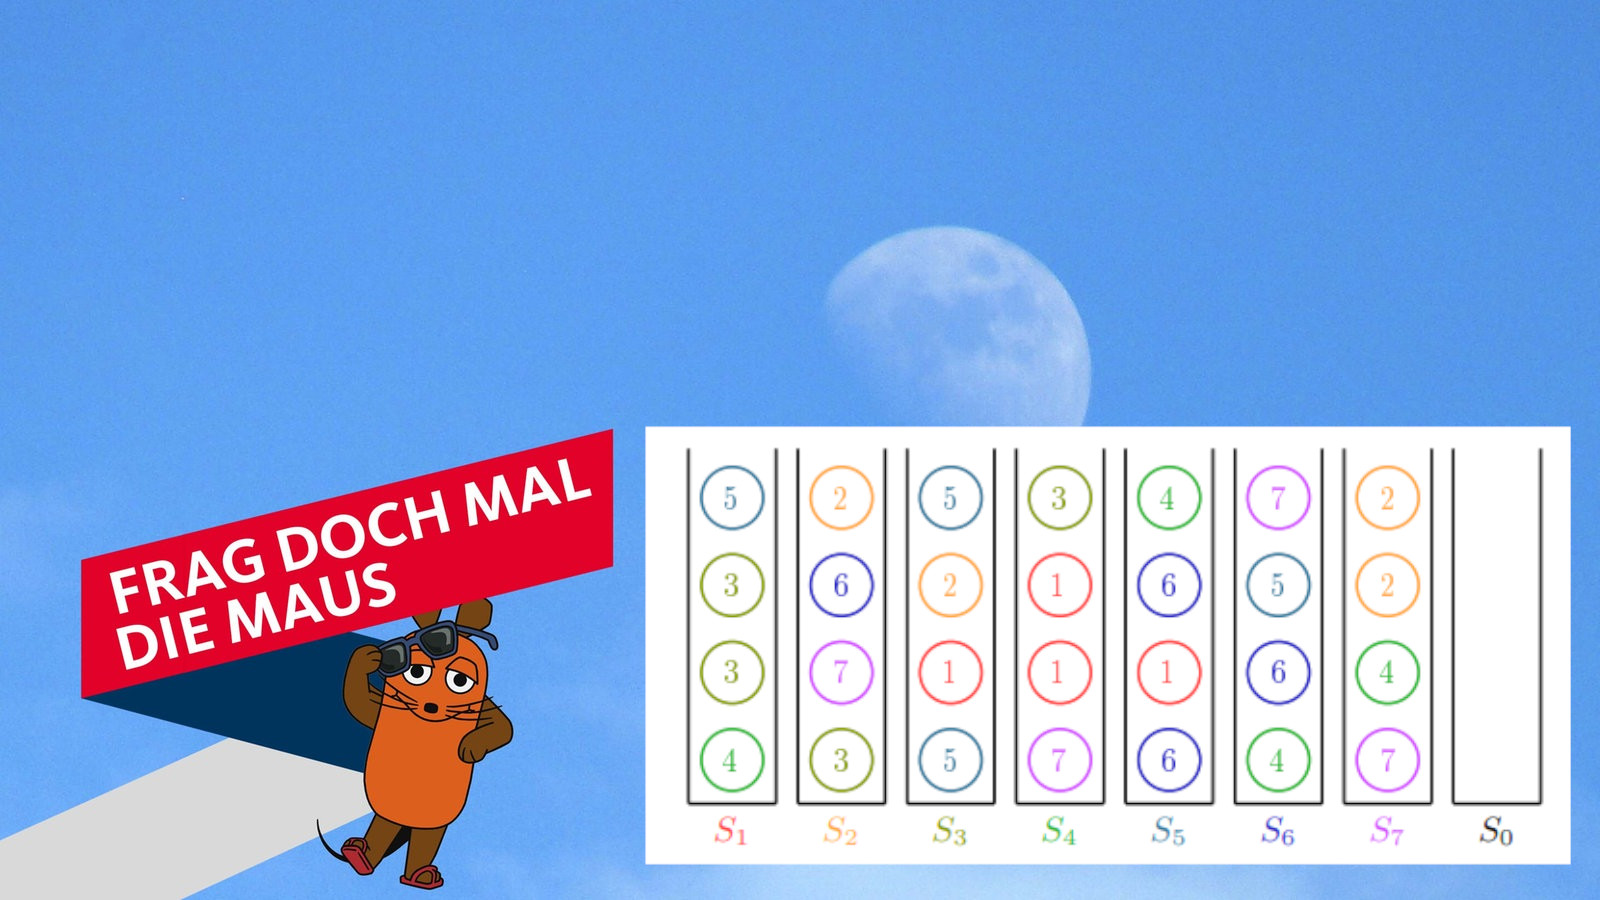
\includegraphics[width=\textwidth]{maus}
    \end{figure}
\end{frame}

\begin{frame}{Idee}
	\begin{pointlist}
		\item Feedback Arc Set Problem (FAS) ist ähnlich zum Spiel mit unbegrenzter Höhe
		\item Konstruktion des Spiels (SCBT) als Graphen 
		\item Reduktion des Problems auf FAS
		\item FAS ist NP-vollständig, somit auch SCBT
	\end{pointlist}
\end{frame}

\begin{frame}{Definitionen}
	\begin{pointlist}
		\item Menge an Farben $C=\{1,\dots c\}$ mit festem $c\in \mathbb{N}$
		\item $c+1$ Tuben der Höhe $h_i\in\mathbb{N}$ in den Farben und eine farblos
		\item Bis zu $h_i$ Bälle pro Farbe
		\item Konfiguration $S$ einer Tube ist eine Sequenz $(b_1,\dots,b_l)$ mit $l\leq h$
		\item Tube-Rack $(T_0, T_1,\dots,T_c)$ hat Höhenprofil $H=(h_0,\dots,h_c)$ und Ersatztube $T_0$
		\end{pointlist}
		\end{frame}
\begin{frame}{Definitionen}
	\begin{pointlist}
		\item Konfiguration eines Tube-Racks ist $S=(S_0,\dots,S_c)$ mit $|S_i| \leq h_i$
		\item Zug $(i,j)$ heißt valide, falls $|S_i|\geq 1$ und $|S_j| < h_j$
		\item Finale Konfiguration ist $S=(S_0,\dots, S_0)$ mit $S_0 = ()$ und $S_i =(i,\dots,i)$ für $1\leq i \leq c$
		\item $i$-farbiger Ball ist in finaler Position, falls er in Tube $i$ ist und alle Bälle darunter Farbe $i$ haben
	\end{pointlist}
\end{frame}

\begin{frame}{Probleme}
	\begin{pointlist}
		\item SCBT-Problem:
		\begin{arrowlist}
 			\item Instanz $(H,S,k)$ mit $k$ validen Zügen
		\end{arrowlist}
		\item Restricted SCBT-Problem (RSCBT):
		\begin{arrowlist}
 			\item Anzahl Bälle der Farbe $i$ gleich der Höhe $h\in\mathbb{N}$ mit dem Höhenprofil $H=(h,\dots,h)$
		\end{arrowlist}
	\end{pointlist}
\end{frame}

\begin{frame}{Lemma 1}
\begin{enumlist}
\item Falls die Anzahl der Bälle der Farbe $i$ $h$ entspricht für alle $1 \leq i \leq c$, hat $((h,\dots,h),S,c\cdot h\cdot (2h+1))$ eine Lösung, 
\item Falls $(H,S,k)$ eine Lösung hat und $H' \geq H$ gilt, dann hat $(H',S,k)$ auch eine Lösung
\item Falls $(H,S,k)$ mit $H=(\infty,\dots, \infty)$ eine Lösung hat, dann existiert eine Lösung mit: \begin{pointlist}
\item Bälle in finaler Position werden nicht bewegt
\item Jeder andere wird 1- oder 2-mal bewegt
\end{pointlist}
\item Falls $((\infty, \dots,\infty),S,k)$ eine Lösung hat und $H=(\infty, h_1,\dots, h_c)$ mit $h_i \geq \max(|s_i|,b_i)$ gilt, dann hat $(H,S,k)$ eine Lösung
\end{enumlist}
\end{frame}

\begin{frame}{Feedback Arc Set (FAS)}
\begin{pointlist}
\item geg.: gerichteter Multigraph G=(V,E) und $k\in\mathbb{N}_0$
\item ges.: $\exists E' \subseteq E$ mit $|E'|\leq k$, sodass $G'(V,E\backslash E')$ azyklisch ist
\begin{arrowlist}
\item Nach Karp (1972) NP-vollständig
\end{arrowlist}
\end{pointlist}
\end{frame}

\begin{frame}{Konstruktion}
\begin{pointlist}
\item $V=\{1,\dots,n\}$ und $G$ azyklisch mit $c=n$
\begin{arrowlist}
\item Eine Tube $S_u$ für jeden Knoten $u\in V$
\item Ein Ball der Farbe $u$ in Tube $v$ Für jede Kante $(u,v)\in E$
\item konstruierte Instanz $((\infty, \dots, \infty), (S_u)_{u=1}^n, |E|+k)$
\end{arrowlist}
\end{pointlist}
\end{frame}

\begin{frame}{Konstruktion}
\begin{figure}[ht]
		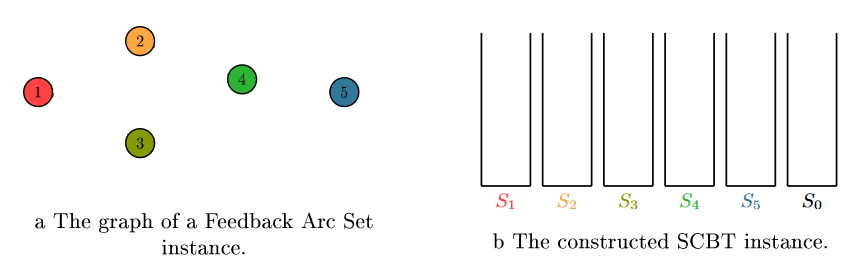
\includegraphics[width=\textwidth]{construct01}
		\caption{Konstruktion}
    \end{figure}
\end{frame}

\begin{frame}{Konstruktion}
\begin{figure}[ht]
		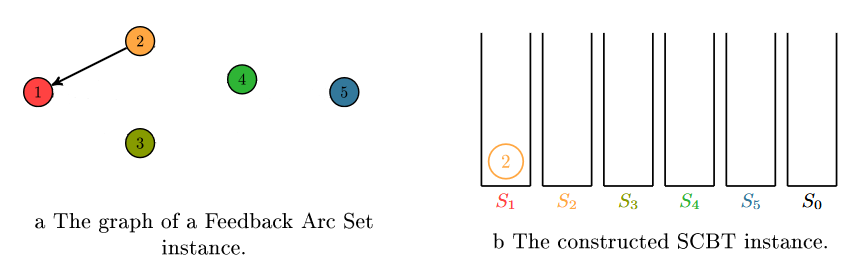
\includegraphics[width=\textwidth]{construct02}
		\caption{Konstruktion}
    \end{figure}
\end{frame}

\begin{frame}{Konstruktion}
\begin{figure}[ht]
		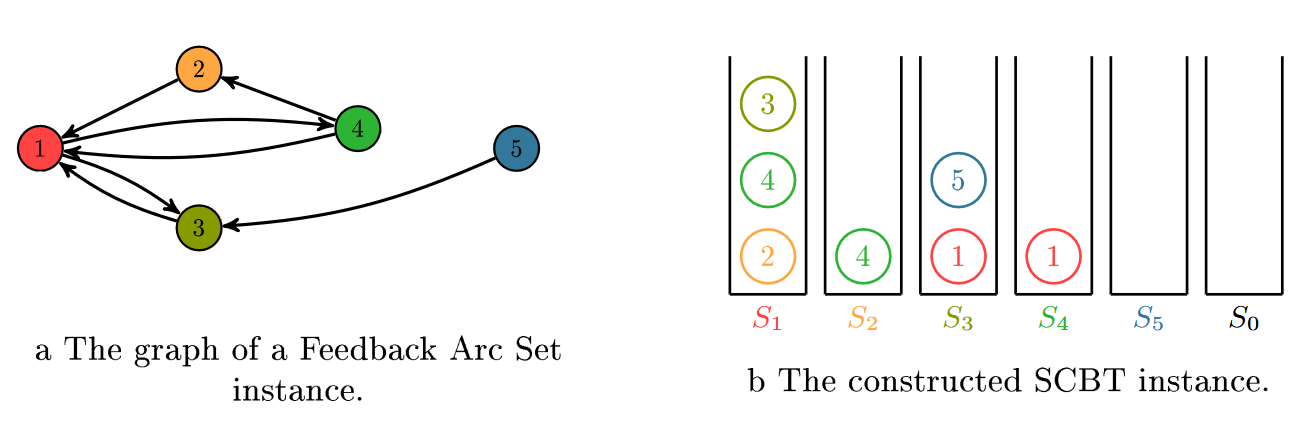
\includegraphics[width=\textwidth]{construct03}
		\caption{Konstruktion}
    \end{figure}
\end{frame}

\begin{frame}{Konstruktion}
\begin{figure}[ht]
		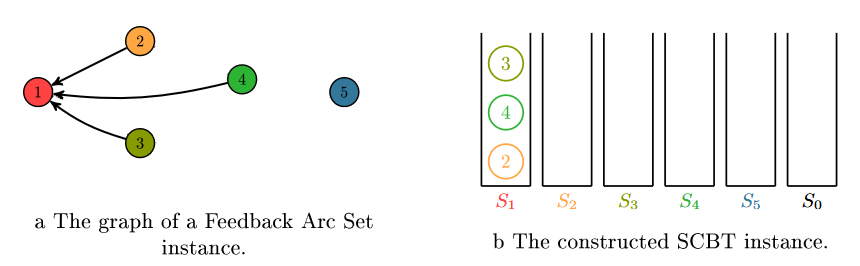
\includegraphics[width=\textwidth]{construct04}
		\caption{Konstruktion}
    \end{figure}
\end{frame}

\begin{frame}{Konstruktion}
\begin{figure}[ht]
		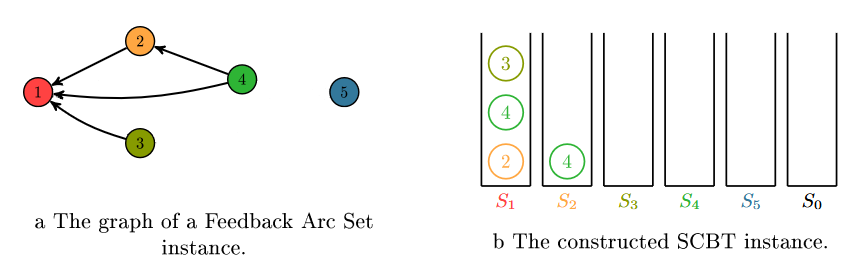
\includegraphics[width=\textwidth]{construct05}
		\caption{Konstruktion}
    \end{figure}
\end{frame}

\begin{frame}{Konstruktion}
\begin{figure}[ht]
		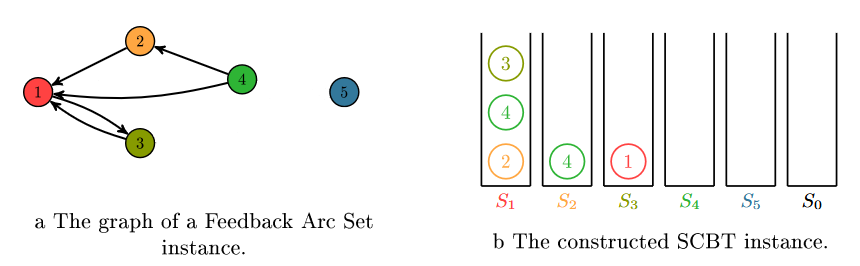
\includegraphics[width=\textwidth]{construct06}
		\caption{Konstruktion}
    \end{figure}
\end{frame}

\begin{frame}{Konstruktion}
\begin{figure}[ht]
		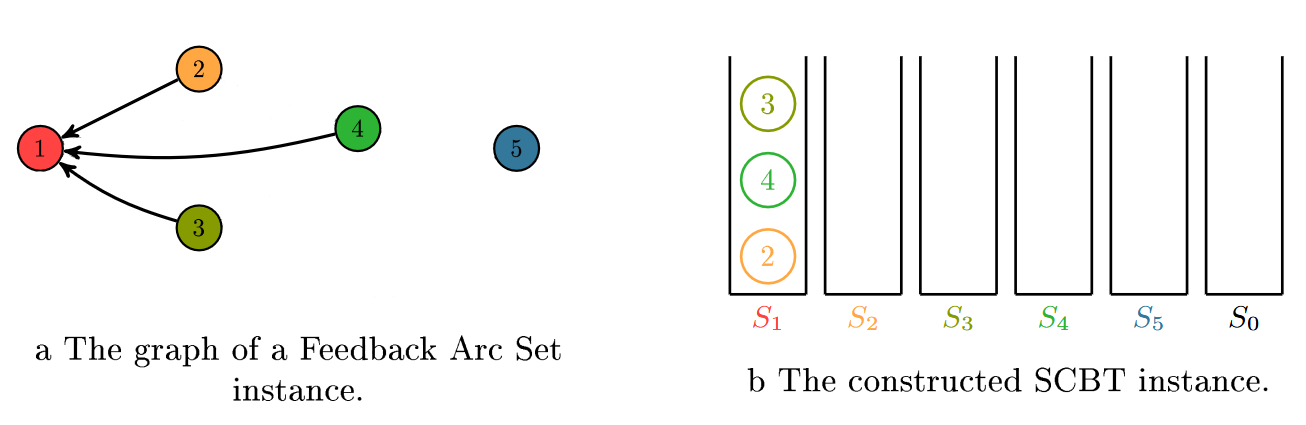
\includegraphics[width=\textwidth]{construct07}
		\caption{Konstruktion}
    \end{figure}
\end{frame}

\begin{frame}{Konstruktion}
\begin{figure}[ht]
		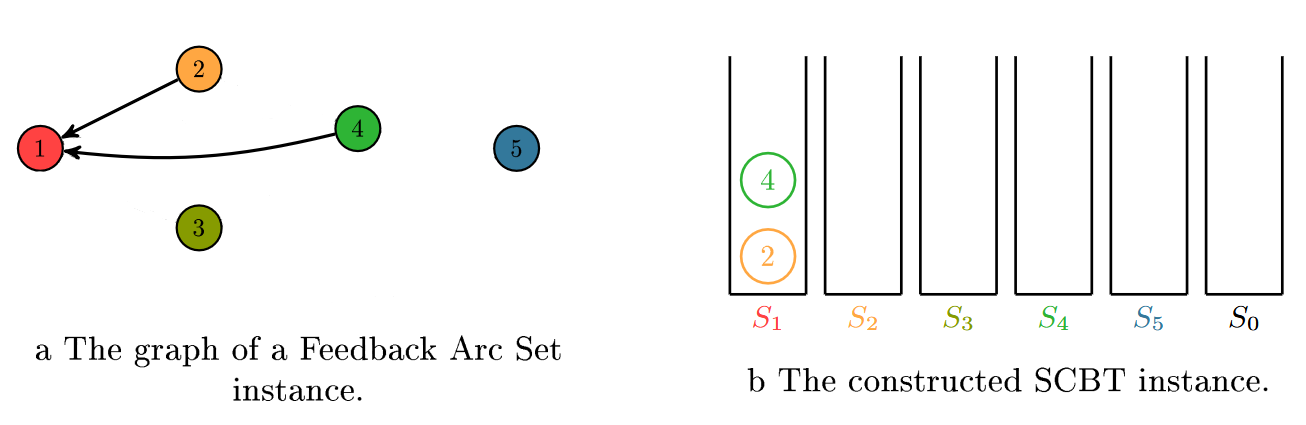
\includegraphics[width=\textwidth]{construct08}
		\caption{Konstruktion}
    \end{figure}
\end{frame}

\begin{frame}{Konstruktion}
\begin{figure}[ht]
		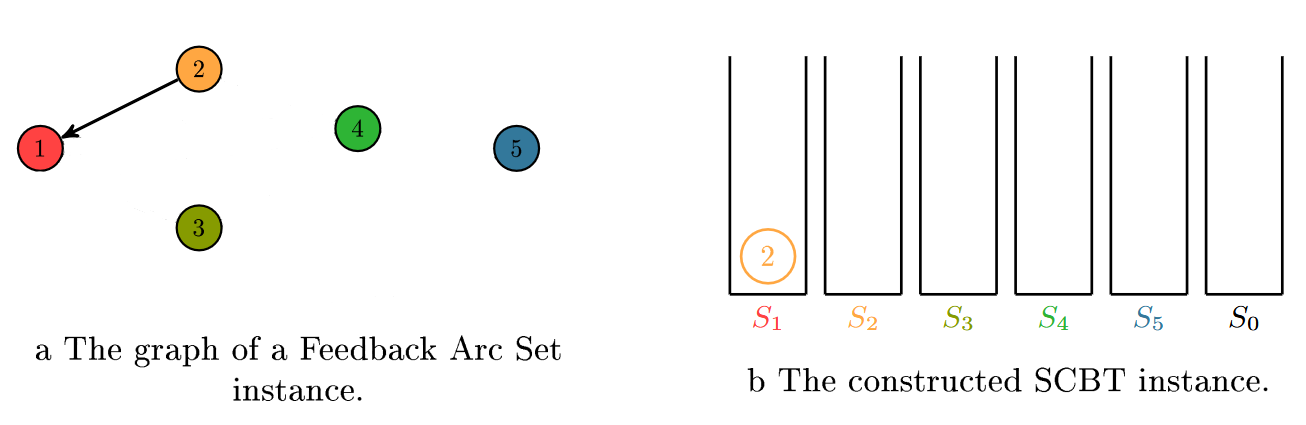
\includegraphics[width=\textwidth]{construct09}
		\caption{Konstruktion}
    \end{figure}
\end{frame}

\begin{frame}{Konstruktion}
\begin{figure}[ht]
		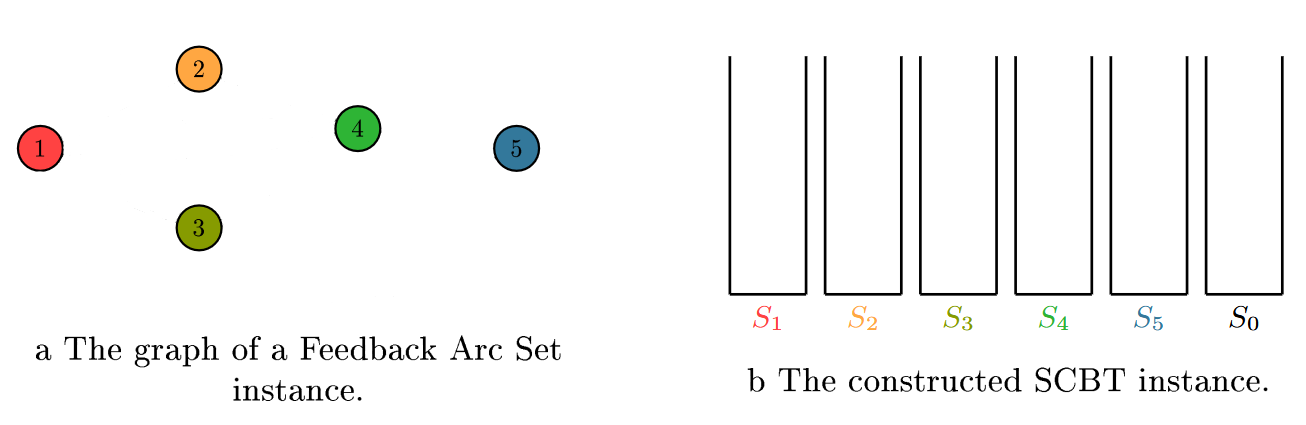
\includegraphics[width=\textwidth]{construct10}
		\caption{Konstruktion}
    \end{figure}
\end{frame}

\begin{frame}{Konstruktion}
\begin{figure}[ht]
		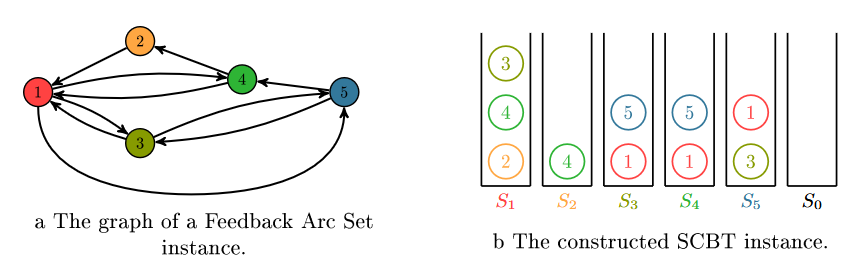
\includegraphics[width=\textwidth]{construct}
		\caption{Konstruktion}
    \end{figure}
\end{frame}

\begin{frame}{Lemma 2}
\begin{pointlist}
\item Instanz $(G,k)$ von FAS hat genau dann eine Lösung, wenn die konstruierte Instanz $((\infty, \dots, \infty), (S_u)_{u=1}^n, |E|+k)$ von SCBT eine Lösung hat
\begin{arrowlist}
\item SCBT ist auch NP-vollständig
\end{arrowlist}
\end{pointlist}
\end{frame}

\begin{frame}{Beweis (\glqq $\Rightarrow$\grqq)}
\begin{pointlist}
\item geg.: $(G,k)$ mit $G=(V,E)$
\item Sei $E'\subseteq E$ mit $|E'| \leq k$ eine Lösung für FAS
\item Sei $\pi:\{1,\dots,n\}\rightarrow \{1,\dots,n\}$ eine topologische Sortierung von $G'=(V, E\backslash E')$, sodass $\forall (u,v)\in E\backslash E': \pi(u)\leq \pi(v)$ 
\item Für $i=1,\dots,n$:
\begin{arrowlist}
\item Bälle in $S_{\pi(i)}$, die einer Kante $(\pi(i),u)\in E\backslash E'$ entsprechen, gehen in Tube $S_u$
\item Bälle in $S_{\pi(i)}$, die einer Kante aus $E'$ entsprechen, gehen in die Reserve-Tube 
\end{arrowlist}
\item Durch die topologische Sortierung ist die Tube $S_u$ die finale für den jeweiligen Ball, daher $k_1 = |E\backslash E'|$ viele Züge
\item Die Bälle in der Reserve-Tube werden schließlich auf ihre Farben aufgeteilt, , daher $k_2 = 2\cdot |E'|$ viele Züge
\item $k_1 + k_2 =  |E\backslash E'| + 2\cdot |E'| = |E| + |E'| \leq |E| + k$
\item Konstruierte Instanz $((\infty, \dots, \infty), (S_u)_{u=1}^n, |E|+k)$ hat eine Lösung
\end{pointlist}
\end{frame}

\begin{frame}{Beweis (\glqq $\Leftarrow$\grqq)}
\begin{pointlist}
\item geg.: Konstruierte Instanz kann in $|E|+k$ Zügen gelöst werden
\item Lemma 1. besagt, dass jeder Ball entweder einmal final bewegt wird oder zuerst in die Reserve-Tube geht
\item Sei $E'$ die Menge mit Bällen, die 2-mal bewegt werden
\item Jeder Ball muss mindestens 1-mal bewegt werden, somit $|E|$
\item Jeder zusätzlicher Zug fällt unter $k$, daher $|E'|\leq k$
\end{pointlist}
\end{frame}

\begin{frame}{Beweis (\glqq $\Leftarrow$\grqq)}
\begin{pointlist}
\item Annahme: $G'=(V,E\backslash E')$ hat einen Zyklus
\item Ball für Kante $(u,v)\in E\backslash E'$ kann erst final bewegt werden, wenn alle Bälle in Zielröhre $S_u$ entfernt wurden
\item Der Ball kann nur bewegt werden, wenn ein anderer im Zyklus bewegt werden kann $\lightning$ 
\begin{arrowlist}
\item $G'=(V,E\backslash E')$ ist azyklisch 
\end{arrowlist}
\end{pointlist}
\end{frame}

\begin{frame}{Definition DFVS}
\end{frame}

\begin{frame}{Lower Bounds}
\end{frame}

\begin{frame}{Algorithmus}
\end{frame}

\begin{frame}{Related Work}
	\begin{pointlist}
		\item Sortieren von farbigen Bällen in farblosen Tuben. Bälle nur auf Bälle gleicher Farbe oder in leere Tuben (Reduktion von 3-Partition)
	\end{pointlist}
\end{frame}

\begin{frame}{Related Work}
	\begin{pointlist}
		\item $k$ $i$-farbige Bälle in umgekehrter Reihenfolge. Nur adjazente Bälle können getauscht werden 
	\end{pointlist}
	\begin{figure}[ht]
		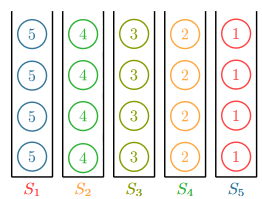
\includegraphics[width=.65\textwidth]{relatedwork}
		\caption{Konstruktion}
    \end{figure}
\end{frame}

\begin{frame}{Related Work}
	\begin{pointlist}
		\item Reales Problem: Container in Terminalen
	\end{pointlist}
	\begin{figure}[ht]
		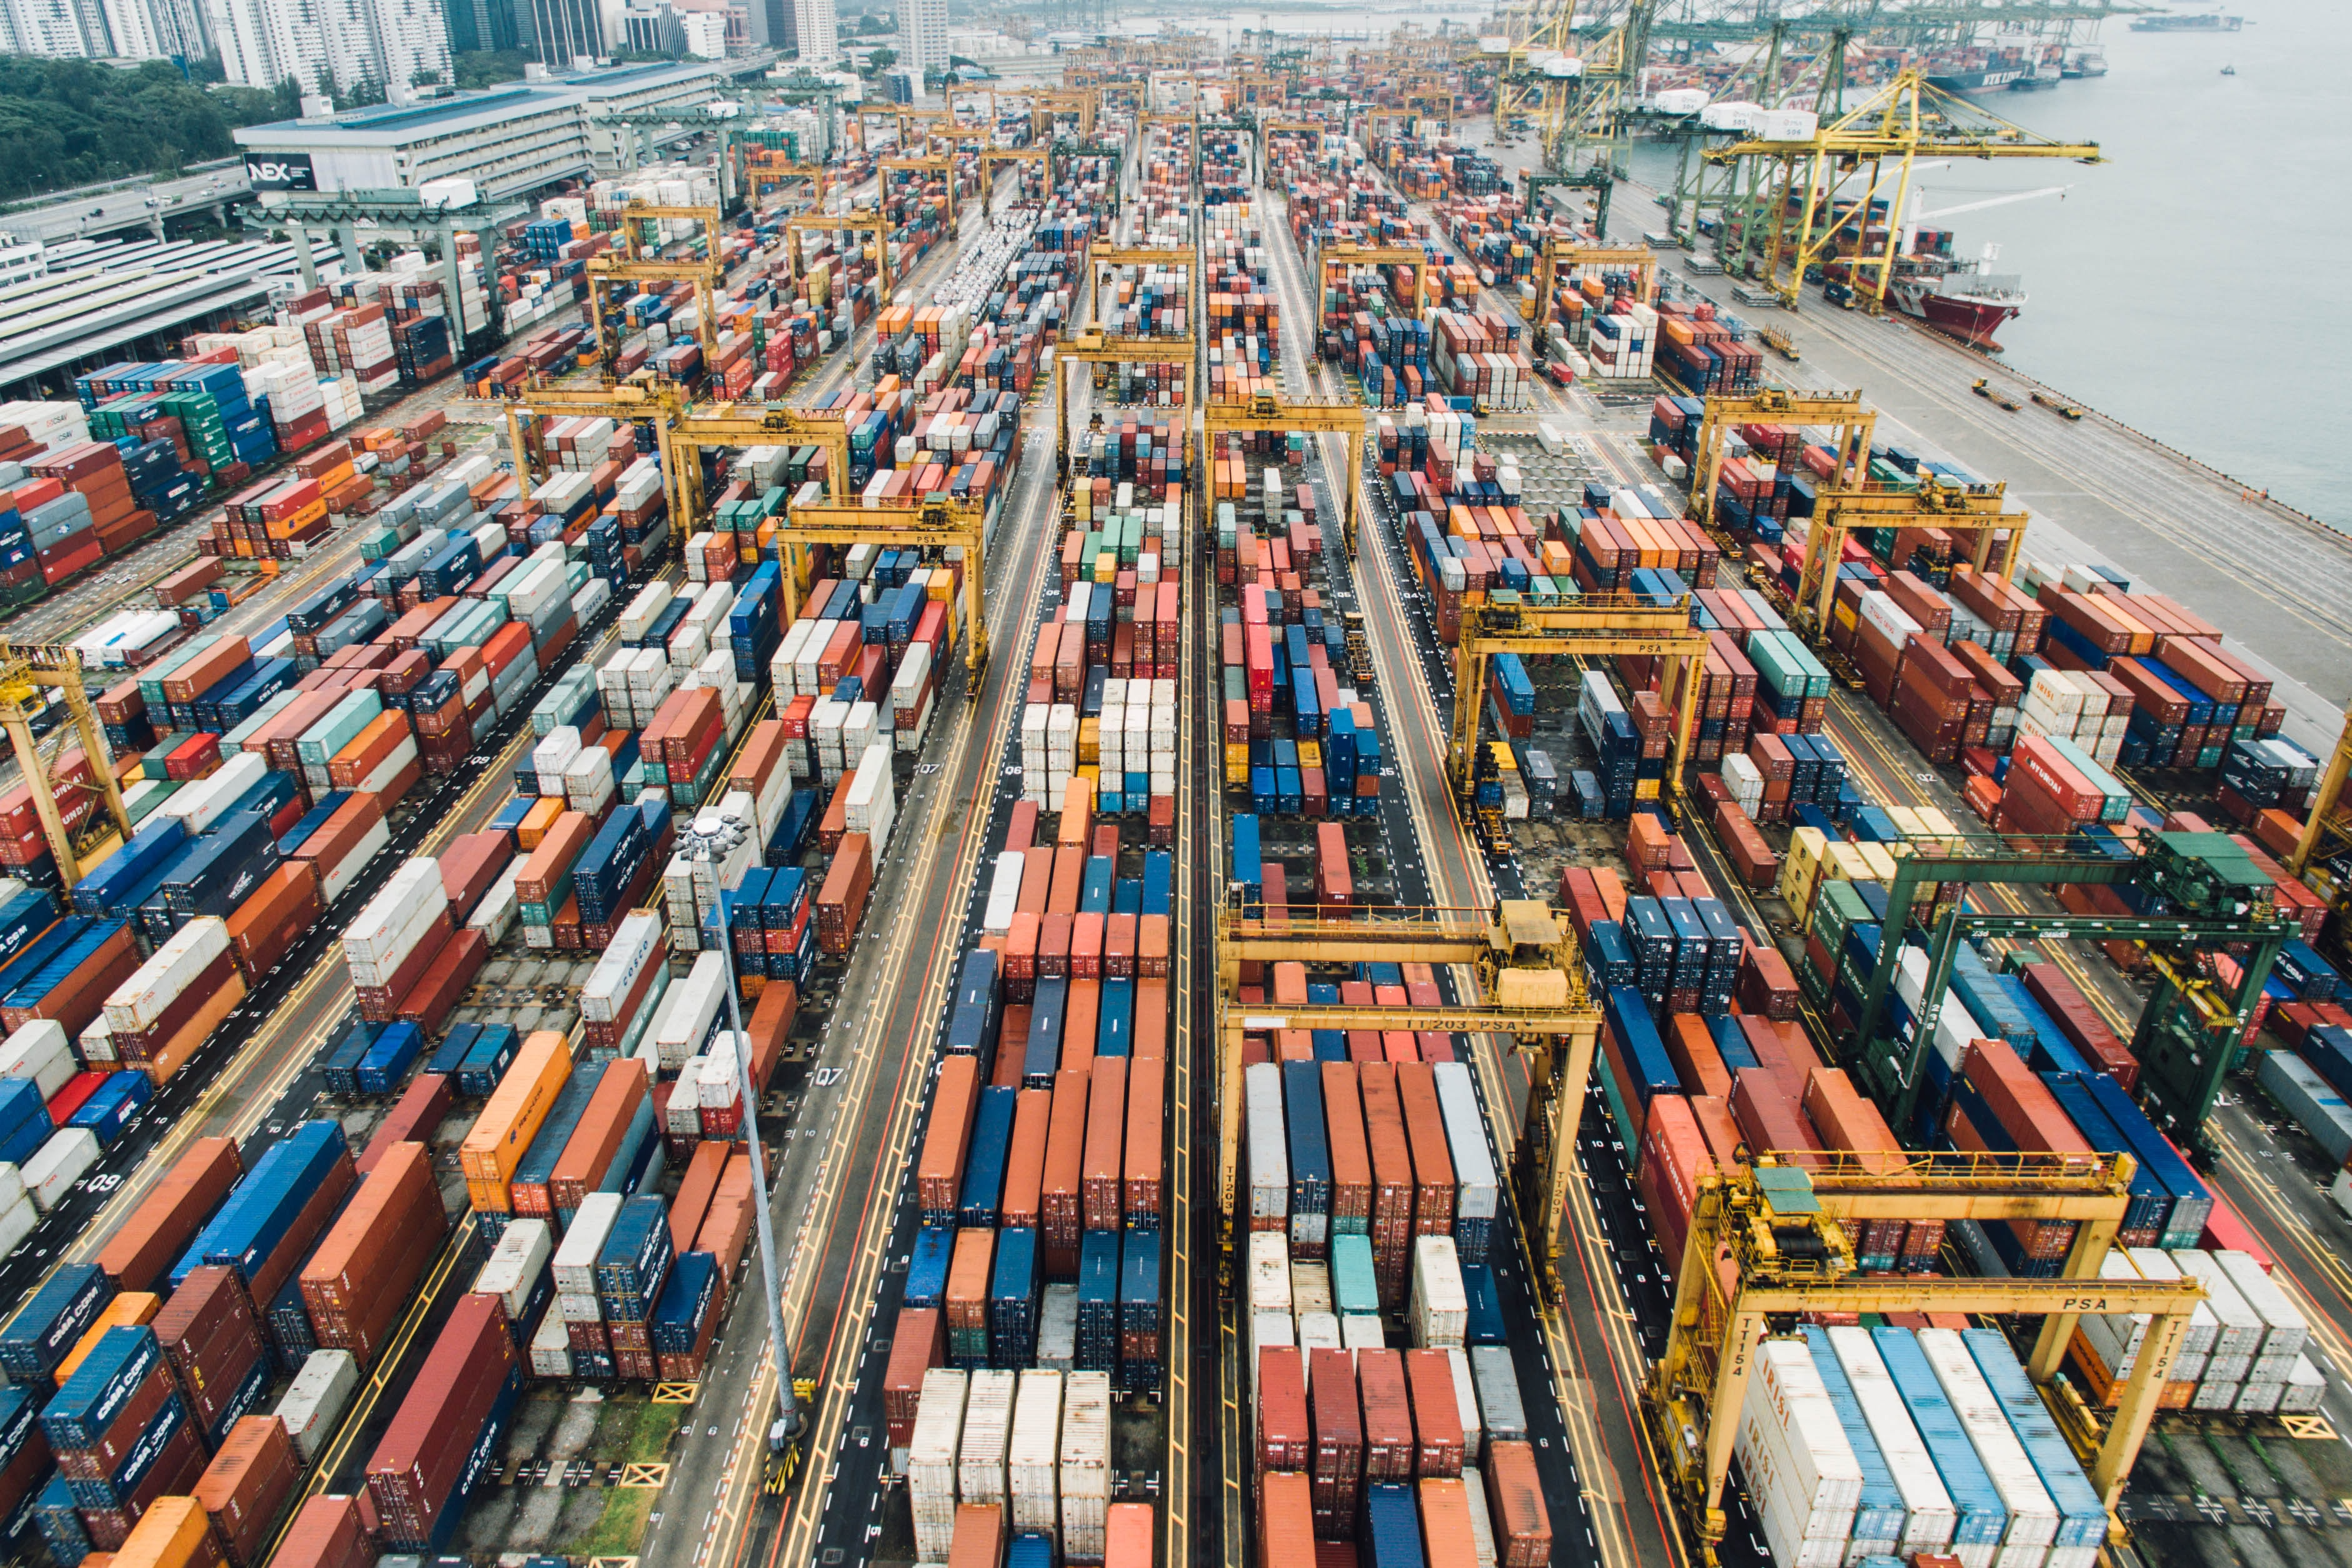
\includegraphics[width=.65\textwidth]{container}
		\caption{Container Terminal}
    \end{figure}
\end{frame}



\begin{frame}{}
  \centering \Huge
  \emph{Fin}
\end{frame}


	
    	
    	
    	
\end{document}
